\documentclass[14pt, a4paper]{extarticle}
\usepackage[utf8]{inputenc}
\usepackage[T2A]{fontenc}
\usepackage[a4paper,
left=2cm,
right=2cm,
top=2cm,
bottom=2cm]{geometry}
\usepackage{color}
\usepackage{mathtools}
\usepackage{listings}
\usepackage{graphicx}
\usepackage{tocloft}
\usepackage{indentfirst}
\usepackage{enumitem}
\usepackage[russian]{babel}
\usepackage[utf8]{inputenc}
\usepackage[russian]{babel}

\usepackage{diagbox}

\setlength{\parindent}{0.8cm}
\setlength{\parskip}{0.4cm}
\renewcommand{\contentsname}{}
\renewcommand{\cftsecleader}{\cftdotfill{\cftdotsep}}
\definecolor{dkgreen}{rgb}{0,0.6,0}
\definecolor{gray}{rgb}{0.5,0.5,0.5}
\definecolor{mauve}{rgb}{0.58,0,0.82}

\lstset{frame=none,
  language=Python,
  aboveskip=3mm,
  belowskip=3mm,
  showstringspaces=false,
  columns=flexible,
  basicstyle={\small\ttfamily},
  numbers=none,
  numberstyle=\tiny\color{gray},
  keywordstyle=\color{blue},
  commentstyle=\color{dkgreen},
  stringstyle=\color{mauve},
  breaklines=true,
  breakatwhitespace=true,
  tabsize=4
}

\title{}
\author{}
\date{}

\begin{document}
  \begin{titlepage}
    \begin{center}
      {\bfseries МИНИСТЕРСТВО НАУКИ И ВЫСШЕГО ОБРАЗОВАНИЯ \\
        РОССИЙСКОЙ ФЕДЕРАЦИИ}
      \\
      Федеральное государственное автономное образовательное учреждение высшего образования
      \\
      {\bfseries «Национальный исследовательский Нижегородский государственный университет им. Н.И. Лобачевского»\\(ННГУ)
        \\Институт информационных технологий, математики и механики} \\
    \end{center}

    \vspace{8em}

    \begin{center}
      ОТЧЕТ \\ по практике \\
      «Идентификация функции конкурентоспособности методами машинного обучения на основе динамики спроса»
    \end{center}

    \vspace{5em}


    \begin{flushright}
      {\bfseries Выполнил:} студент группы\\382006-1\\Мусин А.Н \underline{\hspace{3cm}} \linebreak\linebreak\linebreak
      {\bfseries Проверил:} доцент, к.ф.-м.н.\\ Кузенков О.А.\underline{\hspace{3cm}} 
    \end{flushright}


    \vspace{\fill}

    \begin{center}
      Нижний Новгород\\2024
    \end{center}

  \end{titlepage}

  \tableofcontents
  \thispagestyle{empty}
  \newpage

  \pagestyle{plain}
  \setcounter{page}{3}

  \section{Введение}
  Товар является центральным объектом на рынке, обладающим определенной
  потребительской ценностью, качеством, техническим уровнем, надежностью и
  прочими важными характеристиками. Несмотря на разнообразие аналогов,
  покупатель должен выбрать продукт, который лучше всего соответствует
  его потребностям, учитывая все характеристики. 
  
  Конкуренция,
  фундаментальное понятие в современной экономике, представляет собой
  борьбу между товарами за право существования на рынке, стимулируя
  производителей к улучшению продукции для удовлетворения потребностей
  клиентов.
  
  Конкурентоспособность определяется способностью товара превзойти
  аналоги по техническим, экономическим и эксплуатационным
  характеристикам, что поддерживает его на рынке. Это сравнение с
  конкурентами выявляет наилучший и наихудший варианты с точки зрения
  потребительских предпочтений. Анализ рынка и оценка
  конкурентоспособности товаров становятся ключевыми задачами для
  производителя, который может использовать различные методики, включая
  машинное обучение, для выявления преимуществ и недостатков своей
  продукции.
  
  Методы машинного обучения эффективны для анализа объемных данных,
  выявления тенденций и прогнозирования в условиях динамичного рынка.
  Предложенный в работе подход к использованию машинного обучения для
  прогнозирования конкурентоспособности товара и выявления предпочтений
  покупателей подчеркивает ограниченность современного экономического
  подхода, основанного на линейной зависимости параметров товара.
  \newpage

  \section{Постановка задачи}
  Цель данного исследования заключается в применении методов машинного обучения для определения функции конкурентоспособности на основе изменения спроса. Для достижения этой цели мы начнем с анализа существующих экономических методик оценки конкурентоспособности, близких к теме исследования, с целью выявления их преимуществ и недостатков.

  Далее мы разработаем и обоснуем новый метод расчета функции конкурентоспособности, используя методы машинного обучения, ранжирование и анализ динамики спроса.
  
  Применяя наш метод к рейтингу видеокарт с платформы Steam за период с 2017 по 2024 год, мы восстановим функцию конкурентоспособности товаров.
  
  После этого мы определим значения функции конкурентоспособности для каждой модели, чтобы оценить их потенциальные позиции на рынке. В ходе исследования мы покажем, что функция конкурентоспособности не может быть представлена как линейная комбинация.

  \newpage


  \section{Экономические подходы в оценки конкурентоспособности товаров}
  В настоящее время применяются различные методики оценки
  конкурентоспособности, которые успешно используются в практике
  предприятий и товаров. Каждая из этих методик имеет свои преимущества в
  различных сценариях, однако они также обладают существенными
  недостатками, которые могут привести к ошибочным результатам в данной
  задаче.
  
  В связи с этим необходимо провести анализ существующих методик, выявив
  их сильные и слабые стороны. Только после этого можно предложить
  собственный метод, учитывающий выявленные недостатки.
  
  Одной из методик, используемой в оценке конкурентоспособности, является
  дифференциальный метод. Его суть заключается в анализе отдельных
  (технических и экономических) параметров рассматриваемой продукции и их
  сопоставлении с потребностями. При использовании этого метода можно
  определить, достигла ли продукция необходимого уровня по всем
  параметрам, выявить параметры, которые не соответствуют требованиям, и
  выделить те из них, которые сильнее всего отличаются от базовых.

  \subsection{Дифференциальный метод оценки конкурентоспособности}
  \begin{enumerate}
    \item Если в качестве отправной точки для оценки используются стандартные показатели качества товаров, то расчет единичного показателя конкурентоспособности выполняется с применением следующей формулы:
    \[
    q_{ni} = 
    \begin{cases} 
    0, & \text{если } P_i < P_{i0}, \\
    1, & \text{если } P_i \geq P_{i0} \quad i = 1, 2, \ldots, n 
    \end{cases}
    \]
    
    Где \( q_{ni} \) -- единичный параметрический показатель конкурентоспособности по \( i \)-му нормативному параметру;

    \( P_i \) -- величина \( i \)-го параметра для анализируемой продукции;

    \( P_{i0} \) -- величина \( i \)-го параметра для изделия, принятого за норму;

    \( n \) -- количество параметров;
    
    При использовании нормативных параметров единичный показатель оценки может быть всего лишь двух видов -- 1 или 0. В случае соответствия анализируемой продукции установленным нормам и стандартам, показатель принимает значение 1, в то время как при отклонении параметров продукции от установленных норм и стандартов, показатель становится равным 0.


    \item Если мы принимаем степень удовлетворения потребностей потребителя в
    качестве базового критерия для оценки конкурентоспособности товаров,
    то расчет единичного показателя конкурентоспособности производится с
    использованием следующей формулы:
    \[
    q_{i} = P_{i}/P_{i0}*100\% i = 1,2, \ldots , n
    \]
    \[
      q'_{i} = P_{i0}/P_{i}*100\% i = 1,2, \ldots , n
    \]
    Где \(q_{i}\), \(q'_{i}\) — единичный параметрический показатель конкурентоспособности по i-му нормативному параметру;
    
    \( P_i \) -- величина \( i \)-го параметра для анализируемой продукции;

    \( P_{i0} \) -- величина \( i \)-го параметра для изделия, принятого за норму;

    \( n \) -- количество параметров;
    \paragraph[short]{}
    Из предложенных формул выбирается та, в которой увеличению единичного
     показателя соответствует повышение уровня конкурентоспособности.В случае,
     если характеристики исследуемого товара не могут быть
     измерены количественно (например, параметры вкуса, цвета, консистенции, 
     запаха), применяются экспертные методы оценки в баллах. В этом
     случае подвергают оценке в баллах как исследуемый образец, так и базовый.
  \paragraph[short]{}
  Дифференциальный метод оценки конкурентоспособности ограничивается определением уровня конкурентоспособности по отдельному показателю. Он не учитывает важность каждого параметра, влияющего на
     выбор товара потребителем. По этой причине дифференциальные методы оценки конкурентоспособности применяются обычно в двух сценариях: при использовании степени удовлетворения потребности потребителя
     и при оценке соответствия нормативно-технологическим требованиям.
  \end{enumerate}
  \newpage
  \subsection{Комплексный метод оценки конкурентоспособности}

  Комплексный метод оценки конкурентоспособности базируется на использовании различных видов показателей (групповых, обобщенных и интегральных) и сравнении относительных полезных эффектов между анализируемой продукцией и образом. В данном подходе происходит вычисление групповых показателей, учитывающих нормативные, технические и экономические параметры, после чего рассчитывается обобщенный показатель конкурентоспособности продукции относительно потребности, образца или группы образцов.
  
  \[
  I_{NP} = \prod_{i=1}^n q_{ni}
  \]
  
  Где \(I_{NP}\) — групповой показатель конкурентоспособности по нормативным параметрам;
  
  \(q_{ni}\) — единичный показатель конкурентоспособности по \(i\)-му нормативному параметру;
  
  \(n\) — количество параметров;
  
  А групповые показатели по техническим и экономическим параметрам отражают уровень соответствия исследуемой продукции потребностям покупателя по всем техническим характеристикам и соотношение общих затрат потребителя на покупку и использование данного продукта по сравнению с товаром-образцом.
  
  \[
  I_{TP} = \sum_{i=1}^n \alpha_i q_{ni}
  \]
  
  \[
  I_{EP} = \frac{Z}{Z_0}
  \]
  
  Где \(I_{TP}\) — групповой показатель конкурентоспособности по техническим параметрам;
  
  Где \(I_{EP}\) — групповой показатель конкурентоспособности по экономическим параметрам;
  
  \(q_{i}\) — единичный показатель конкурентоспособности по \(i\)-му техническому параметру;
  
  \(\alpha_i\) — весомость \(i\)-ого параметра в общем наборе из \(n\) технических параметров, характеризующих потребность;
  
  \(n\) — число параметров, участвующих в оценке;
  
  \(Z, Z_0\) — полные затраты потребителя соответственно по оцениваемой продукции и образцу.
  
  Интегральный показатель отражает разницу между сравниваемыми товарами в отношении потребительского эффекта, который приходится на каждую единицу затрат покупателя на их приобретение и использование.

  \[
  K = \frac{I_{NP} \cdot I_{TP}}{I_{EP}}
  \]
  
  Где \(K\) — интегральный показатель конкурентоспособности анализируемой продукции по отношению к изделию-образцу;
  
  Соответственно если \(K < 1\), то рассматриваемый товар уступает образцу по конкурентоспособности, а если \(K > 1\), то превосходит. При этом, если, предположим, что \(I_{NP} = 1\), то есть товар полностью соответствует стандартам по всем нормативным параметрам, а \(Z\) — величина постоянная, тогда \(I_{EP}\) — константа, и тогда выражение преобразуется в:
  
  \[
  K = \frac{1}{C_0} \sum_{i=1}^n \alpha_i q_{ni}
  \]
  
  Следовательно, интегральный показатель выражается в виде линейной функции его технических параметров. Однако такая оценка обладает рядом недостатков, например, коэффициенты \(\alpha\) основаны на данных, полученных из социологических опросов группы лиц, и не всегда отражают объективную реальность. Это может создать проблемы при корректности построении функции конкурентоспособности. С другой стороны, подход к оценке конкурентоспособности товаров, вдохновленный работами Кузенкова О.А., Морозова А.Ю., Кузенковой Г.В., Рябовой Е.А., Гарсиа А., подчеркивает сложность с приспособляемостью живых существ. В свете этих исследований становится ясным, что линейная модель не всегда является приемлемой для построения функции приспособляемости. Иногда необходим переход к сверткам более высоких порядков. Исходя из этого, мы переходим к разработке новой методологии.
  
  \section{Методика расчета конкурентоспособности}

  Допустим, имеется \( l \) различных видов товаров с аналогичным предназначением, обозначенных как \( v_1, v_2, \ldots, v_l \). Обозначим их множество как \( D \). Для каждого товара \( v \) в момент времени \( t_k \), где \( k = 1, \ldots, n \), существует величина \( x(v, t_k) \), представляющая количество данного товара, приобретенное потребителем в текущий момент времени \( t_k \). Все значения \( x(v, t_k) \) неотрицательны, а вектор \( x(v|t) = (x(v, t_0), \ldots, x(v, t_n)) \) характеризует общее состояние системы.
  
  Объем спроса зависит от предпочтений покупателей, цен и характеристик товаров. Предположим, что цены на товары не изменяются со временем. Таким образом, объем спроса \( x(v, t) \) на товар \( v \) определяется исключительно предпочтениями покупателей. Мы предполагаем, что \( x(v, t) \) соответствует определенным свойствам:
  \begin{enumerate}
      \item \( x(v, t) = 0 \) означает отсутствие \( v \) на рынке в момент времени \( t \);
      \item \( x(v, t) > 0 \) означает наличие \( v \) на рынке в момент времени \( t \);
      \item \( x(v, t) \) является непрерывной функцией \( v \) в \( D \);
      \item \( x(v, t) \) является непрерывной функцией времени \( t \);
      \item стремление к нулю \( x(v, t) \) со временем означает угасание объемов продаж;
      \item \( x(v, t) \) равномерно ограничена константой, т.е. \( x(v, t) < C \) – ограничение на максимальное возможное число товаров на рынке.
  \end{enumerate}
  
  Формально ранжирование товаров можно определить следующим образом. Модель \( v \) лучше, чем модель \( w \), если:
  \[
  \lim_{t \to \infty} \frac{x(w, t)}{x(v, t)} = 0
  \]
  Это утверждение означает, что с течением времени (при \( t \to \infty \)) спрос на модель \( w \) вытесняется с рынка. Таким образом, мы вводим порядок ранжирования в множество \( D \).
  
  Предположим, что существует функционал \( J(v) \), который сохраняет ранжирование моделей. Мы можем рассматривать его как функцию сравнения, то есть
  \[
  J(v) > J(w) \Leftrightarrow v > w
  \]
  где выражение \( v >> w \) интерпретируется как "модель \( v \) превосходит модель \( w \)". Тогда предложенный функционал может быть идентифицирован как мера конкурентоспособности товара.
  
  Математически, существование введенной функции конкурентоспособности подчиняется требованиям, соответствующим теореме Дебре о непрерывности. Для этого предполагается, что товары удовлетворяют критериям рациональности (соответствуют логике и потребностям потребителя, обладают высоким качеством, адекватной ценой и выполняют свою функцию в соответствии с целями приобретения) и непрерывности (доступны для приобретения и использования в любое удобное для клиента время, то есть всегда доступны без временных или иных местных ограничений, мешающих их приобретению). В таком случае функция \( J \) является непрерывной.

  Из этой постановки следует, что товар \( v^* \), при котором функция конкурентоспособности достигает максимума, будет оптимальным, поскольку эта модель в конечном итоге вытеснит все другие, занимая самую значительную долю рынка.
  
  Общий объем спроса на рынке в момент \( t_k \) обозначим \( u(t_k) = \sum_{i=1}^l x(v_i, t_k) \). Эта величина может принимать различные значения в зависимости от \( t_k \), но при этом справедливы неравенства \( 0 < u_0 \leq u(t_k) \leq u_1 \), где \( u_0, u_1 \) – положительные константы – минимальное и максимальное значения общего объема спроса соответственно. Величина \( z(v_i, t_k) = \frac{x(v_i, t_k)}{u(t_k)} \) является удельным весом i-го товара на рынке в момент времени \( t_k \).
  
  Итак \( z(v_i, t_k) \) удельный вес величины спроса i-го товара в момент времени \( t_k \), который вычисляется из статистических данных спроса. Время рассматриваем дискретное.
  
  \[
  \Delta z(v_i, t_0) = z(v_i, t_0 + (k+1)\Delta t) - z(v_i, t_0 + (k+1)\Delta t)
  \]
  
  \noindent Как было показано в работах О.А Кузенкова характеристика спроса, которая так же является показателем конкурентоспособности вычисляется следующим способом:
  
  \[
  J(v_i) =< ln(1+\frac{\Delta z(v_i, t_k)}{z(v_i, t_k)}) >= \frac{1}{n} \sum_{i=1}^n ln(1+\frac{\Delta z(v_i, t_k)}{z(v_i, t_k)})
  \](1.0)
  
  Сравнивая обнаруженные значения для каждого товара, можно выяснить, который из них более конкурентоспособен.
  
  Для каждой модели \( v \) динамика спроса \( x(v, t) \) определяется различными потребительскими, коммерческими и экономическими параметрами. Предположим, что общее количество таких параметров равно \( m \). Тогда этот набор можно представлять в виде вектора \( M(v) = (M_1(v), M_2(v), \ldots, M_m(v)) \). Конкурентоспособность \( J \) является функцией многих переменных от \( M(v) \), то есть \( J = J(M(v)) \).
  
  Далее предположим, что функция \( J \) является достаточно гладкой функцией параметров \( M_i \). Таким образом, мы можем аппроксимировать \( J \) с использованием разложения Тейлора вокруг некоторой точки \( M_0 \). В частности, мы можем рассмотреть приближение функции приспособленности в классе линейных или квадратичных функций путем свертки параметров. Ранее уже было сказано, что линейная свертка не всегда является уместной, поэтому в данной работе ключевая роль отводится сверткам более высоких порядков. В данном примере рассматривается квадратичная:
  
  \[
  J(M) = \sum_{i=1}^m \lambda_i M_i(v) + \sum_{i=1}^m \sum_{j=1}^m \lambda_{ij} M_i(v) M_j(v)
  \]
  
  где \( \lambda_i, \lambda_{ij} \) - степени влияния каждого признака на общую конкурентоспособность, \( M_i \) - i-ая характеристика модели, \( M_iM_j \) - произведение i-ой и j-ой характеристики.
  
  В случае когда товар v лучше, чем w должно выполняться неравенство \( J(v) > J(w) \), соответственно коэффициенты \( \lambda_k \) должны удовлетворять неравенству:
  
  \[
  \sum_{i=1}^m \lambda_i(M_i(v) - M_i(w)) + \sum_{i=1}^m \sum_{j=1}^m \lambda_{ij} (M_i(v) M_j(v) - M_i(w) M_j(w)) > 0
  \]
  
  Таким образом, каждая пара стратегий порождает аналогичное неравенство. Решая эту систему неравенств, можно оценить параметр \( \lambda \), например, с применением линейного программирования. Однако размерность данной задачи может быть в общем случае чрезвычайно большой, и поэтому компоненты, входящие в неравенства, могут быть вычислены приближенно. Это может привести к небольшим погрешностям при решении, что, в свою очередь, может вызвать несовместность системы.

Для преодоления упомянутых трудностей мы прибегаем к попарному подходу ранжирования, используя машинное обучение для определения коэффициентов. Мы сопоставляем паре \( (v, w) \) точку \( (M(v) - M(w)) \) в многомерном пространстве параметров размерности \( m, n \), а паре \( (w, v) \) - точку \( (M(w) - M(v)) \). Таким образом, мы стремимся к тому, чтобы гиперплоскость вида

\[
\sum_{i=1}^m \lambda_i(M_i(v) - M_i(w)) + \sum_{i=1}^m \sum_{j=1}^m \lambda_{ij}(M_i(v)M_j(v) - M_i(w)M_j(w)) = 0
\]

разделяла эти точки. Рассматривая все возможные пары точек, мы получаем два множества точек в \( m, t \)-мерном пространстве, находящихся по разные стороны от разделяющей гиперплоскости.

Задача поиска параметра \( \lambda \) сводится к нахождению компонентов нормали гиперплоскости, разделяющей два множества точек. Эта задача сводится к бинарной классификации, которую можно легко решить с использованием специализированных методов машинного обучения. В частности, метод опорных векторов (SVM) хорошо зарекомендовал себя в таких задачах.

Метод опорных векторов (SVM) принимает входные данные для двух классов и возвращает коэффициенты разделяющей гиперплоскости. Основная цель алгоритма заключается в поиске оптимальной гиперплоскости, которая эффективно разделяет данные на два класса.

Алгоритм устроен таким образом, что он выявляет точки, расположенные ближе всего к гиперплоскости разделения, и такие точки называются опорными векторами. Затем алгоритм вычисляет расстояние между опорными векторами и самой разделяющей плоскостью, которое называется зазором. Основная задача алгоритма заключается в максимизации этого зазора.

Лучшей гиперплоскостью считается та, которая максимально удалена от скопления точек каждого класса. Таким образом, алгоритм стремится найти гиперплоскость с максимальным зазором, обеспечивая максимальное расстояние между классами и, следовательно, повышая эффективность разделения.


  \section{Реализация}
  \subsection{Сбор данных}
  В качестве динамики спроса на графические процессоры возьмем открытые данные игровой платформы Steam по популярности видеокарт среди геймеров.
  Роль игроков в видеоигры для рынка графических процессоров (GPU) является значительной и многогранной. Геймеры не только являются основными потребителями высокопроизводительных GPU, но также существенно влияют на развитие технологий и тенденций в данной индустрии. Рассмотрим несколько ключевых аспектов этой роли:

  \begin{enumerate}
  \item\textbf{Спрос на производительность.}
  Геймеры требуют высокопроизводительных GPU для обеспечения плавного и качественного игрового опыта. Современные игры становятся все более графически насыщенными и требовательными к ресурсам, что стимулирует спрос на мощные графические карты.
  \item\textbf{Обновление оборудования.}
  Игроки регулярно обновляют свои GPU, чтобы соответствовать новым стандартам и требованиям игр, что поддерживает постоянный спрос на новейшие модели видеокарт.
  \item\textbf{Разработка новых технологий.}
  Для удовлетворения запросов геймеров производители GPU, такие как NVIDIA и AMD, разрабатывают новые технологии, включая трассировку лучей (ray tracing), улучшенные алгоритмы сглаживания и прочие графические улучшения.
  \item\textbf{Конкуренция.}
  Высокий спрос на игровые GPU приводит к усиленной конкуренции между производителями, что ускоряет технологический прогресс и улучшает качество продукции.
  \item\textbf{Оптимизация игр.}
  Производители GPU активно работают с разработчиками игр для оптимизации игр под свои графические карты, что обеспечивает лучший игровой опыт и стимулирует продажи как игр, так и GPU.
  \item\textbf{Поддержка технологий.}
  Многие современные игры включают поддержку технологий, разработанных производителями GPU, таких как NVIDIA DLSS (Deep Learning Super Sampling) или AMD FSR (FidelityFX Super Resolution), что улучшает производительность и качество изображения.
  \item\textbf{Обзоры и рекомендации.}
  Геймеры активно делятся отзывами и рекомендациями о графических картах, влияя на решения других покупателей. Популярные геймеры и стримеры имеют значительное влияние на рынок, продвигая определенные модели GPU.
  \item\textbf{Киберспорт.}
  Развитие киберспорта также стимулирует спрос на высокопроизводительные GPU, так как профессиональные игроки требуют максимальной производительности для достижения успеха в соревнованиях.
  \item\textbf{Продажи и доходы.}
  Игровой сегмент является одним из самых прибыльных для производителей GPU. Продажи игровых видеокарт составляют значительную долю доходов таких компаний, как NVIDIA и AMD.
  \item\textbf{Инвестиции в R\&D.}
  Доходы от продаж игровых GPU позволяют компаниям инвестировать в исследования и разработки, что ведет к созданию новых продуктов и улучшению существующих технологий.
  \end{enumerate}

  Геймеры играют ключевую роль в формировании и развитии рынка GPU. Их требования и ожидания стимулируют инновации, поддерживают высокие объемы продаж и оказывают значительное влияние на стратегии и решения производителей графических процессоров.

  В качестве характеристик возьмем открытую базу данных с результатами исполнения специальных тестов (бенчмарков). \\\\
  \textbf{Бенчмарки} (от англ. "benchmark") — это тесты производительности, предназначенные для оценки и сравнения аппаратного и программного обеспечения. В контексте видеокарт, бенчмарки используются для измерения производительности графических процессоров (GPU) в различных задачах, таких как рендеринг игр, обработка графики, выполнение вычислений и т.д.\\\\
  \textbf{Почему бенчмарки важны для сравнения видеокарт:}
  \begin{enumerate}
    \item\textbf{Объективное сравнение производительности} Бенчмарки предоставляют стандартный способ измерения производительности видеокарт, позволяя объективно сравнивать различные модели. Это особенно важно для геймеров, разработчиков и профессионалов, которые зависят от графической мощности для своей работы.
    \item\textbf{Реальные сценарии использования} Хорошие бенчмарки включают тесты, имитирующие реальные условия использования, такие как запуск современных игр или выполнение профессиональных графических задач. Это позволяет пользователям понять, как видеокарта будет вести себя в условиях, близких к их реальным потребностям.
    \item\textbf{Проверка стабильности и надёжности} Помимо производительности, бенчмарки могут выявить потенциальные проблемы с перегревом, стабильностью и совместимостью видеокарт. Это важно для долгосрочной надежности и безопасности системы.
    \item\textbf{Сравнение по различным параметрам} Бенчмарки могут измерять производительность видеокарт по различным аспектам, таким как частота кадров (FPS) в играх, время рендеринга в графических приложениях, производительность в вычислительных задачах и т.д. Это дает комплексное понимание сильных и слабых сторон каждой видеокарты.
  \end{enumerate}
  \textbf{Примеры популярных бенчмарков для GPU}\\
  В данной работе будут фигурировать характеристики основанные на двух популярных бенчмарках:
  \begin{enumerate}
    \item\textbf{Vulkan} Специализированный тест на архитектуре Vulkan.
    \item\textbf{OpenCV} Специализированный тест на архитектуре OpenCV.
    \item\textbf{3DMark} Один из самых популярных и универсальных бенчмарков, используемый для тестирования игровых и профессиональных видеокарт.
    \item\textbf{2DMark} Специализированный тест, который включает сценарии, моделирующие использование профессиональных графических приложений, таких как Adobe Illustrator или AutoCAD, для оценки производительности в 2D-графике.
  \end{enumerate}
  Также рассматривается характеристика цены актуальная на момент сбора данных (февраль 2022г.) И метрика тепловыделения видеокарты (TDP). Однако так как все параметры должны положительно коррелировать с приспособленностью товара возьмем обратные величины. Далее везде будут использованы величины равные \(1/price\) и \(1/TDP\).
  
  \paragraph{}
  Данные приведены в приложении (2).
  \paragraph{}
  Эти данные разделим на тренировочные и тестовые в пропорции 70 на 30. В дальнейшем все восстановление функции происходит на тренировочных данных. На тестовых проверяется результат.

  \newpage
  \section{Восстановление функции конкурентоспособности с помощью линейных параметров.}
Для начала взглянем на графическое представление наших данных:
\begin{figure}[h]
  \centering
  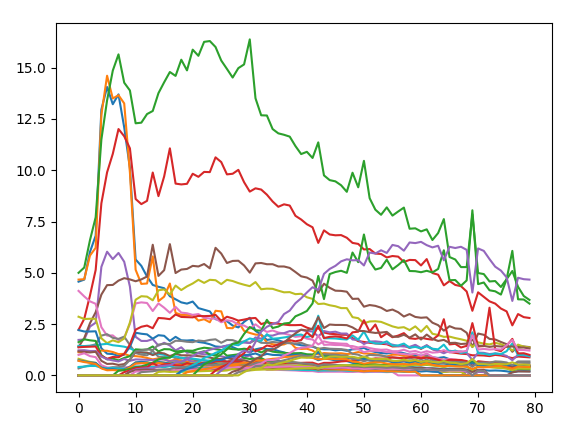
\includegraphics[width=0.8\textwidth]{./img/linear/graph-data.png}
  \caption{Динамика рынка GPU (2017-2024гг).}
  \label{fig:example}
\end{figure}
\newline
На данном графике можно увидеть типичные ситуации вытеснения товаров на рынке, что характерно для нашей теории.
\newpage
Далее посмотрим на матрицу корреляции линейных характеристик и параметра J высчитанного по формуле 1.0.
\begin{figure}[h]
  \centering
  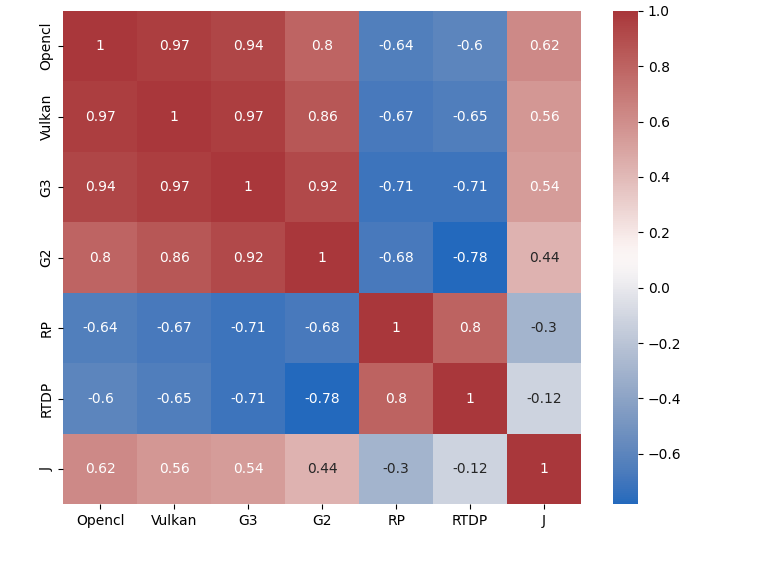
\includegraphics[width=0.8\textwidth]{./img/linear/corr.png}
  \caption{Матрица корреляции характеристик.}
  \label{fig:example}
\end{figure}
\newline
Как мы можем увидеть корреляция между параметрами достаточно высокая. Значение посчитанной конкурентоспособности достаточно сильно коррелирует с остальными параметрами, что дает надежду на лучшее восстановление. Однако, для машинного обучения сильная корреляция губительна. Для того чтобы перейти к следующему этапу
необходимо избавиться от нее. С данной задачей может справиться метод главных компонент (PSA).
\paragraph{}
Перейдем непосредственно к решению. В дальнейшем мы будем работать со стандартизированными данными. Для этого для каждой характеристики посчитаем среднее выборочное (Мат. Ожидание) и среднеквадратичное отклонение.
После чего найдем стандартизированные значения характеристик по формуле:
\[
  z_i = \frac{x_i - \mu}{\sigma}
\]


\textbf{Mетод главных компонент.} Применяя для новых данных метод главных компонент получим преобразованные данные и матрицу коэффициентов метода главных компонент, обозначим ее {W}.
\newline

\begin{figure}[h]
  \centering
  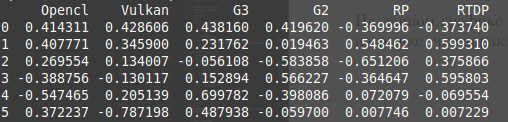
\includegraphics[width=0.8\textwidth]{./img/linear/w-matrix.png}
  \caption{Матрица W.}
  \label{fig:example}
\end{figure}

\begin{figure}[h]
  \centering
  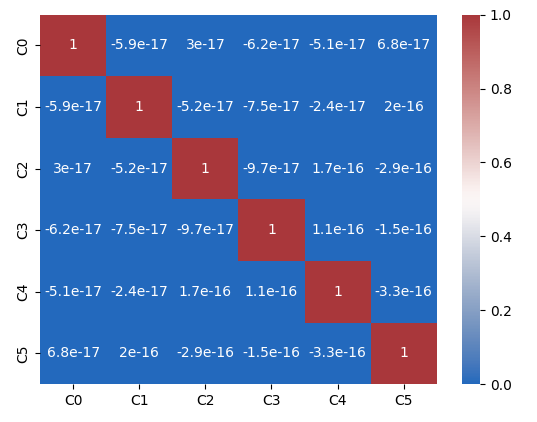
\includegraphics[width=0.8\textwidth]{./img/linear/psacorr.png}
  \caption{Матрица корреляции в главных компонентах.}
  \label{fig:example}
\end{figure}
\paragraph{}

Корреляция в главных компонентах отсутствует. Можно переходить к машинному обучению.
\paragraph{}

\textbf{Mашинное обучение.} Для решения задачи регрессии будем исследовать всевозможные пары объектов. Для начала сравним их и разделим на классы по принципу описанному выше. Если посчитанная конкурентоспособность объекта А больше чем у объекта В то отнесем их к 1-му классу. Если меньше то ко 2-му.
Также исключим граничные случаи. Для этого введем параметр \(\mathcal{E}\). Если \(\left|J_i - J_j\right| < \mathcal{E}\) то пара \(i, j\)
не участвует в обучении. 
\newpage
\paragraph{}
Далее для каждой пары объектов найдем метрики обучения. Данные метрики будут представлять собой разности между значениями главных компонент.
\[
  M^k_{ij} = C_{i}^{k} - C_{j}^{k},  k = 1, ... , n
\]
Где \(n\) - количество главных компонент.
\paragraph{}
Для реализации будем использовать метод опорных векторов (SVM). Результатом работы данного алгоритма будут коэффициенты разделяющей гиперплоскости. Обозначим их как вектор V. 
\begin{figure}[h]
  \centering
  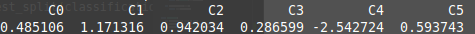
\includegraphics[width=0.8\textwidth]{./img/linear/vectorv.png}
  \caption{Вектор V.}
  \label{fig:example}
\end{figure}
\paragraph{}
Данные коэффициенты задают гиперплоскость в пространстве опорных векторов. Для того чтобы перейти к пространству начальных характеристик умножим данный вектор слева на матрицу W.
Получим вектор коэффициентов начальных характеристик. Обозначим его C.
\[
  C = W \times V
\]
\begin{figure}[h]
  \centering
  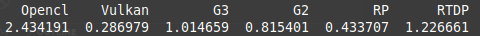
\includegraphics[width=0.8\textwidth]{./img/linear/vectorc.png}
  \caption{Вектор C.}
  \label{fig:example}
\end{figure}
\paragraph{}
Данные коэффициенты являются коэффициентами восстановленной функции конкурентоспособности. Сама функция выглядит следующим образом:
\[
  J = \sum_{i=1}^n C_i \frac{N_i - \mu_i}{\sigma_i}
\]
\(N_i\) - значение i-ой характеристики
\newline
\(\mu_i\) - значение мат ожидания посчитанного на обучающих данных.
\newline
\(\sigma_i\) - значение среднеквадратичного отклонения посчитанного на обучающих данных.
\newline
\(C_i\) - i-й восстановленный коэффициент.
\newpage
\textbf{Тестирование.} Тестирование восстановленной функции будет происходить на тестовых данных.
Для этого возьмем данные в порядке уменьшения посчитанной конкурентоспособности и посчитаем значение восстановленной функции для этих объектов.
Далее два списка объектов (отсортированные по посчитанной и восстановленной функции) будут сравниваться друг с другом.
\paragraph{}
\textbf{Алгоритм сравнения.} Значение данного теста будет число $t \in [0, 1]$ которое обладает следующими свойствами:
\begin{enumerate}
  \item\textbf{При t = 0} Объекты идут в обратном порядке.
  \item\textbf{При $t \in (0, 0.5)$} Большинство объектов соблюдает обратный порядок.
  \item\textbf{При $t = 0.5$} Объекты идут в случайном порядке.
  \item\textbf{При $t \in (0.5, 1)$} Большинство объектов соблюдает порядок.
  \item\textbf{При t = 1} Порядок полностью соблюдается.
\end{enumerate}
\paragraph{}
Чем ближе число t к 1 тем лучше восстановлена динамика данных.
\paragraph{}
Для функции с характеристиками взятыми линейно t = 0.6, что говорит о плохом восстановлении функции. Как раньше говорилось в описании метода такой результат может быть связан с нелинейным влиянием характеристик на конкурентоспособность товара.
\newline
\section{Увеличение размерности.}
Для дальнейшей реализации алгоритма предлагается оптимизировать обучающую выборку. Для этого введем алгоритм восстановления:

Параметры алгоритма:
\begin{enumerate}
  \item\textbf{\(\mathcal{E}\)} -- Параметр контролирующий минимальную разницу между посчитанными значениями функции конкурентоспособности чтобы это сравнение вошло в выборку. 
  \item\textbf{Z (мес.)} -- Параметр минимального времени нахождения товара на рынке. (Если товар находится на рынке меньше Z месяцев товар не участвует в обучении)
  \item\textbf{D (dimention)} -- Порядок вхождения параметров.
\end{enumerate}
\paragraph{}
\begin{enumerate}
    \item На основании параметра D для каждого объекта берутся всевозможные произведения характеристик порядка от 1 до D. Эти значения становится новыми характеристиками.
    \item На основании параметра Z выбираются объекты выборки находящиеся на рынке не менее Z месяцев, которые становятся новой обучающей выборкой.
    \item К данной выборке применяется метод главных компонент. Количество главных компонент равно количеству характеристик.
    \item Составляется обучающая выборка машинного обучения состоящая из пар объектов. Однако на основании параметра E если разница между значениями конкурентоспособности меньше E то пара не попадает в выборку.
    \item Происходит восстановление параметров \(\lambda\). И тестирование на обучающей выборке. Значение вышеприведенного теста (t) является выходным параметром метода.
\end{enumerate}
\paragraph{}
Далее предлагается используя алгоритм оптимизации (в данной работе будет использоваться алгоритм дифференциальной эволюции) найти максимум данной функции. 
\paragraph{}
\textbf{Результаты работы алгоритма оптимизации на приведенных данных: \(\mathcal{E}\) = 0.002, Z = 28, D = 4. Значение теста на обучающей выборке 0.72.}
\paragraph{}
Далее необходимо проверить результат на тестовой выборке.
\paragraph{}
Значение на тестовой выборке \textbf{0.805.} Данный результат говорит о хорошем восстановлении функции.

\paragraph{}
Посчитанные коэффициенты функции находятся в приложении 3 к данной работе.
\paragraph{}
\section{Тестирование на реальном примере.}
Возьмем некоторую видеокарту которая не участвовала в обучении и посчитаем ее конкурентоспособность.
\begin{figure}[h]
    \centering
    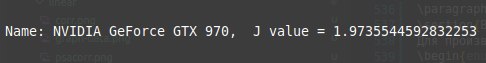
\includegraphics[width=0.8\textwidth]{./img/linear/test_gpu.png}
    \caption{Тестовая GPU и ее посчитанная конкурентоспособность.}
    \label{fig:example}
  \end{figure}
\paragraph{}
Далее посмотрим на ее поведение в некоторой части тестовой выборки отсортированной по значению функции.
\begin{figure}[h]
    \centering
    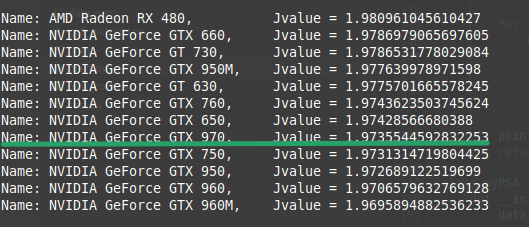
\includegraphics[width=0.8\textwidth]{./img/linear/test_calc.png}
    \caption{Тестовая GPU в выборке. Посчитанная конкурентоспособность.}
    \label{fig:example}
  \end{figure}
\paragraph{}
\newpage
Далее для сравнения посчитаем значение конкурентоспособности по восстановленной функции и отсортируем данные по уменьшению значения.
\begin{figure}[h]
    \centering
    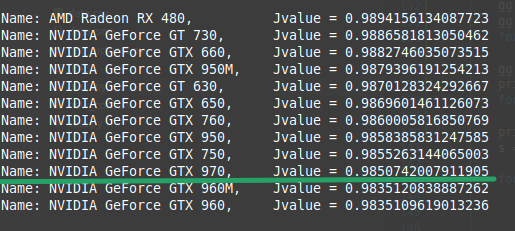
\includegraphics[width=0.8\textwidth]{./img/linear/test_restored.png}
    \caption{Тестовая GPU в выборке. Восстановленная конкурентоспособность.}
    \label{fig:example}
\end{figure}
\paragraph{}
Значение t на данной выборке 85.5\%. Поведение видеокарты на рынке восстановилось достаточно хорошо. Порядок предпочтительности соблюдается. Это позволяет сказать что на основании данной восстановленной функции конкурентоспособности можно с неплохой точностью и на основании доступных данных показать динамику рынка GPU.
\newpage
\section{Возможные применения.}
Для производителей GPU функция конкурентоспособности несомненно имеет множество полезных применений:
\begin{enumerate}
  \item\textbf{Стратегическое планирование}
  \subitem Анализ рынка: Функция предоставляет данные для стратегического анализа рынка, выявления новых возможностей и угроз.
  \subitem Долгосрочное планирование: Помогает в разработке долгосрочных планов по развитию линейки продуктов и технологий.
  \item\textbf{Ценообразование}
  \subitem Определение оптимальной цены: Анализ конкурентоспособности помогает определить справедливую цену для нового продукта, учитывая его производительность по сравнению с продуктами конкурентов.
  \item\textbf{Оптимизация продуктов}
  \subitem Анализ производительности: Производители могут использовать функцию для анализа производительности своих GPU в сравнении с конкурентами. Это помогает выявить слабые и сильные стороны продукта.
  \subitem Таргетирование улучшений: На основе данных о конкурентоспособности можно принять решения о том, какие аспекты GPU требуют улучшения (например, производительность в играх, вычислительные мощности для ИИ, энергоэффективность).

\end{enumerate}
\newpage
\section{Заключение}

В заключение, проведенное исследование продемонстрировало эффективность методов машинного обучения в выявлении функции конкурентоспособности на основе динамики спроса. Анализ существующих экономических методик позволил выделить ключевые преимущества и недостатки, что послужило основой для разработки нового метода расчета функции конкурентоспособности.

Применение предложенного метода к рейтингу видеокарт с платформы Steam за период с 2017 по 2024 год позволило успешно восстановить функцию конкурентоспособности и определить её значения для каждой модели. Результаты исследования подтвердили, что функция конкурентоспособности не может быть представлена как линейная комбинация, что подчеркивает сложность и многогранность факторов, влияющих на конкурентоспособность товаров.

Таким образом, данная работа вносит значимый вклад в развитие методов оценки конкурентоспособности и открывает новые возможности для применения машинного обучения в экономическом анализе. Полученные результаты могут быть полезны как для научных исследований, так и для практического применения в стратегическом планировании и маркетинговых исследованиях.
\newpage

\section{Приложение}
\subsection{Исходный код Python}
  \subsubsection{main.py}
  \begin{lstlisting}
    import sys
from matplotlib import pyplot as plt
import pandas as pd
import seaborn as sns
import numpy as np

from common.data import GetData, GetTest
from sklearn.decomposition import PCA

from sklearn import svm
from sklearn.model_selection import train_test_split
from sklearn.metrics import accuracy_score
from sklearn.datasets import load_iris
from sklearn.metrics import confusion_matrix
from colorama import Fore
from scipy.optimize import differential_evolution





ZERO_NUM = 0
ERROR = 0.0
DIM = 0



class DataManager:
    data = GetData(ZERO_NUM, DIM)
    test = GetTest(ZERO_NUM, DIM)
    
    @classmethod
    def get_statistic_df(cls):
        res = pd.DataFrame([dict(i.get_stats()) for i in cls.data]).T
        res.columns = [i.get_name() for i in cls.data]
        return res

    @classmethod
    def get_metrics_df(cls):
        return pd.DataFrame([i.get_metrics() for i in cls.data])

    @classmethod
    def get_united_metrics_df(cls):
        return pd.DataFrame([i.get_united_metrics() for i in cls.data])

    @classmethod
    def get_united_metrics_val(cls):
        return np.array([i.get_united_metrics().values() for i in cls.data])

    @classmethod
    def calculate_J_val(cls, c_array, mean, std):
        res = []
        for gpu_ in cls.data:
            metrics = list(gpu_.get_united_metrics().values())
            sum = 0
            for metr_, _ in enumerate(metrics):
                sum+= c_array[metr_]*((metrics[metr_] - mean[metr_])/std[metr_])
            res.append((sum, gpu_.get_Jval()))
        return res

    @classmethod
    def get_united_metric_names(cls):
        return pd.DataFrame(cls.data[0].get_united_metrics().keys())

    @classmethod
    def get_classification_df(cls):
        classification_table = []
        for i in [(gpu.get_name(), gpu.get_Jval()) for gpu in cls.data]:
            row = [i[0]]
            for j in [(gpu.get_name(), gpu.get_Jval()) for gpu in cls.data]:
                if j[0] == i[0]:
                    row.append(0)
                    continue
                if i[1] > j[1]:
                    row.append(-1)
                else:
                    row.append(1)
            classification_table.append(row)
        classificationDF = pd.DataFrame(classification_table, columns=['name']+[gpu.get_name() for gpu in cls.data])
        return classification_table
    
    @classmethod
    def get_training_Y(cls):
        res = []
        gpu_vals = [gpu.get_Jval() for gpu in cls.data]
        gpu_n = len(gpu_vals)
        for i in range(gpu_n):
            for j in range(gpu_n):
                if abs(gpu_vals[i] - gpu_vals[j]) > ERROR:
                    if j == i:
                        pass
                    elif gpu_vals[i] > gpu_vals[j]:
                        res.append(1)
                    elif gpu_vals[i] <= gpu_vals[j]:
                        res.append(-1)
        return res
    
    @classmethod
    def get_training_X(cls, pca_data):
        pca_data = np.array(pca_data)
        res = []
        gpu_n = len(pca_data)
        metric_n = len(pca_data[0])
        for i in range(gpu_n):
            for j in range(gpu_n):
                if abs(cls.data[i].get_Jval() - cls.data[j].get_Jval()) > ERROR:
                    if j == i:
                        pass
                    else:
                        row = []
                        for k in range(metric_n):
                                row.append(pca_data[i][k] - pca_data[j][k])
                        res.append(row)
        return res
    
    @classmethod
    def testing(cls, c_array, mean, std):
        res1 = []
        for gpu_ in cls.test:
            metrics = list(gpu_.get_united_metrics().values())
            sum = 0
            for metr_, _ in enumerate(metrics):
                sum+= c_array[metr_]*((metrics[metr_] - mean[metr_])/std[metr_])
            res1.append((sum, gpu_.get_name()))
        res1.sort(key= lambda x: x[0])

        res=[]
        for gpu_ in cls.test:
            res.append((gpu_.get_Jval(), gpu_.get_name()))
        res.sort(key= lambda x: x[0])
        s = 0
        
        for i in range(len(res)-1):
            k=-1
            for j in range(len(res1)):
                if res1[i][1] == res[j][1]:
                    k = j
                if res[i+1][1] == res1[j][1] and k!=-1:
                    s+=1
        print(f"TESTING ACCURACY: {s/len(cls.test)} ZERO_NUM: {ZERO_NUM}, ERROR: {ERROR}, DIM: {DIM}")
        return s/len(cls.test)

class myPSA:
    def __init__(self, df) -> None:
        data_scaled = np.array(df)
        self.data_scaled = data_scaled
        n_components = min(len(data_scaled[0]), len(data_scaled))
        print(f"Optimal number of components: {n_components}")
        pca = PCA(n_components=n_components)
        self.data_pca = pca.fit_transform(data_scaled)
        self.components = pca.components_

    def get_new_data(self):
        return pd.DataFrame(self.data_pca)

    def get_components(self):
        return self.components


class Regression:
    def __init__(self, data) -> None:
        classification_X = DataManager.get_training_X(data)
        classification_Y = DataManager.get_training_Y()
        
        
        self.X_train, self.X_test, self.y_train, self.y_test = train_test_split(classification_X, classification_Y, test_size=0.01, random_state=0)
        clf = svm.SVC(kernel='linear')
        clf.fit(classification_X, classification_Y)
        y_pred = clf.predict(self.X_test)
        self.coefficients = clf.coef_

        self.accuracy = accuracy_score(self.y_test, y_pred)

    def get_coefficients(self):
        return self.coefficients


class PicturesGenerator:
    @staticmethod
    def get_df_plot(df):
        df.plot(logy=False, legend=False)
        plt.show()
        
    @staticmethod
    def get_df_corr_matrix(df):
        corr = df.corr()
        sns.heatmap(corr, annot=True, cmap='vlag',
                xticklabels=corr.columns.values,
                yticklabels=corr.columns.values)
        plt.show()



class UIController:
    @staticmethod
    def show_graphs():
        statsDF = DataManager.get_statistic_df()
        PicturesGenerator.get_df_plot(statsDF)

        metricsDF= DataManager.get_metrics_df()
        PicturesGenerator.get_df_corr_matrix(metricsDF)

        metricsDF= DataManager.get_united_metrics_df()
        PicturesGenerator.get_df_corr_matrix(metricsDF) 

def array_s(a):
    res = []
    for i in a[0]:
        if i < 0:
            res.append(0)
        else:
            res.append(i)
    return res
def execute(h):
    global ZERO_NUM
    global ERROR
    global DIM
    ZERO_NUM = h[0]
    ERROR = h[1]
    DIM = h[2]
    DataManager.data = GetData(ZERO_NUM, DIM)
    DataManager.test = GetTest(ZERO_NUM, DIM)
    metricsDF= DataManager.get_united_metrics_df()
    scaledMetricsDF = (metricsDF - metricsDF.mean()) / metricsDF.std()
    psa = myPSA(scaledMetricsDF)
    NewData = psa.get_new_data()
    svm = Regression(NewData)
    CompCoeff = psa.get_components()
    SvmCoeff = svm.get_coefficients()
    coefArray = np.abs(np.dot(SvmCoeff, CompCoeff))
    print(coefArray)
    s = pd.DataFrame(coefArray, columns=DataManager.data[0].get_united_metrics().keys())
    print(s)
    coefArray = coefArray[0]
    mean = list(metricsDF.mean())
    std = list(metricsDF.std())
    s = DataManager.calculate_J_val(coefArray, mean, std)
    s.sort(key=lambda x: x[1])
    return 1/DataManager.testing(coefArray, mean, std)
    
    
if __name__ == '__main__':
    print(differential_evolution(execute, bounds=[(0,80), (0, 0.03), (0,4)]))
  \end{lstlisting}
  \subsubsection{data.py}
  \begin{lstlisting}
    from dataclasses import dataclass, asdict
    from typing import List
    from math import log
    from os.path import join, abspath
    from os import getcwd
    
    
    import numpy as np
    DIM = 0
    
    
    @dataclass
    class Metrics:
        Opencl: float
        Vulkan: float
        G3: float
        G2: float
        # reciprocal value 1/val
        RP: float
        RTDP: float
    
    
    @dataclass   
    class Stats:
        stats_list : List
    
    
    class GPU:
        name: str
        stat: list
        metrics: Metrics
    
        def __init__(self, _name, _stat, _metr:Metrics) -> None:
            self.name = _name
            self.stat = _stat
            self.metrics = _metr
            self._2d_metrics = self.get_2d_metrics()
            self._3d_metrics = self.get_3d_metrics()
    
        def get_metrics(self) -> dict:
            return asdict(self.metrics)
        
        def get_3d_metrics(self) -> dict:
            res = {}
            i = 0
            for keya, vala in asdict(self.metrics).items():
                i+=1
                j=0
                for keyb, valb in asdict(self.metrics).items():
                    j+=1
                    k = 0
                    for keyc, valc in asdict(self.metrics).items():
                        k+=1
                        if j >= i and k >= j and k >= i:
                            res[f"{keya}*{keyb}*{keyc}"] = vala*valb*valc
            return res
        
        def get_4d_metrics(self) -> dict:
            res = {}
            i = 0
            for keya, vala in asdict(self.metrics).items():
                i+=1
                j=0
                for keyb, valb in asdict(self.metrics).items():
                    j+=1
                    k = 0
                    for keyc, valc in asdict(self.metrics).items():
                        k+=1
                        m = 0
                        for keyd, vald in asdict(self.metrics).items():
                            m+=1
                            if j >= i and k >= j and m >= k:
                                res[f"{keya}*{keyb}*{keyc}*{keyd}"] = vala*valb*valc*vald
            return res
        
        def get_5d_metrics(self) -> dict:
            res = {}
            i = 0
            for keya, vala in asdict(self.metrics).items():
                i+=1
                j=0
                for keyb, valb in asdict(self.metrics).items():
                    j+=1
                    k = 0
                    for keyc, valc in asdict(self.metrics).items():
                        k+=1
                        m = 0
                        for keyd, vald in asdict(self.metrics).items():
                            m+=1
                            n=0
                            for keye, vale in asdict(self.metrics).items():
                                n+=1
                                if j >= i and k >= j and m >= k:
                                    res[f"{keya}*{keyb}*{keyc}*{keyd}*{keye}"] = vala*valb*valc*vald*vale
            return res
        
        
        def get_2d_metrics(self) -> dict:
            res = {}
            i = 0
            for keya, vala in asdict(self.metrics).items():
                i+=1
                j = 0
                for keyb, valb in asdict(self.metrics).items():
                    j+=1
                    if j <= i:
                        res[f"{keya}*{keyb}"] = vala*valb
            return res
        
        def get_stats(self) -> dict:
            return {i : self.stat[i] for i, _ in enumerate(self.stat)}
    
        def get_name(self):
            return self.name
        
        def get_united_metrics(self) -> dict:
            s = {}
            s.update(asdict(self.metrics))
            if DIM > 1:
                s.update(self.get_2d_metrics())
            if DIM > 2:
                s.update(self.get_3d_metrics())
            if DIM > 4:
                s.update(self.get_5d_metrics())
                
            return s
        
        def get_Jval(self) -> float:
            stats_arr = self.stat
            res = 0
            start_flag = False
            n = 0
            for i in range(len(stats_arr)):
                if stats_arr[i] != 0:
                    start_flag = True
                if not start_flag:
                    continue
                if i == 0: continue
                if stats_arr[i] and stats_arr[i-1]:
                    res += log(1 + ((stats_arr[i]-stats_arr[i-1])/stats_arr[i-1]))
                n+=1
            return res/n + 2
    
    
    
    
    def GetData(zero_num, dim):
        global DIM
        DIM = dim
        with open(join(abspath(join(__file__, '..')), 'ndata.csv'), 'r') as data:
            lines = data.readlines()
        
        res = []
        for line in lines[1:]:
            line = line[:-1]
            spl = line.split(',')
            if spl.count("0") < zero_num:
                res.append(line)
        print(f"len 1 = {len(lines)} len = {len(res)}")
        lines = res
        res_gpu = []
        sum_array = [0 for _ in range(80)]
        for line in lines:
            spl = line.split(',')
            metr = Metrics(float(spl[1]), float(spl[2]), float(spl[3]), float(spl[4]), 1/float(spl[5]), 1/float(spl[6]))
            stat = [float(i) for i in spl[7:]]
            res_gpu.append(GPU(spl[0], stat, metr))
        return res_gpu
    
    def GetTest(zero_num, dim):
        global DIM
        DIM = dim
        with open(join(abspath(join(__file__, '..')), 'ndata.csv'), 'r') as data:
            lines = data.readlines()
        res = []
        for line in lines[1:]:
            line = line[:-1]
            spl = line.split(',')
            res.append(line)
        print(f"TEST len 1 = {len(lines)} len = {len(res)}")
        
        lines = res
        res_gpu = []
        for line in lines:
            spl = line.split(',')
            metr = Metrics(float(spl[1]), float(spl[2]), float(spl[3]), float(spl[4]), 1/float(spl[5]), 1/float(spl[6]))
            stat = [float(i) for i in spl[7:]]
            res_gpu.append(GPU(spl[0], stat, metr))
        return res_gpu
  \end{lstlisting}
  \section{Приложение 2}
\subsection{Исходные данные}
\begin{table}
    \centering
    \scriptsize
    \begin{tabular}{llrrrrrr}
 & Name & Opencl & Vulkan & G3D & G2D & Price & TDP \\
0 & NVIDIA GeForce GTX 960 & 21072 & 22380 & 6042 & 671 & 172.000000 & 120 \\
1 & NVIDIA GeForce GTX 750 Ti & 12954 & 12372 & 3919 & 498 & 88.110000 & 60 \\
2 & NVIDIA GeForce GTX 1060 & 32388 & 31476 & 10070 & 762 & 279.990000 & 120 \\
3 & NVIDIA GeForce GTX 1050 Ti & 22192 & 21230 & 6314 & 651 & 189.420000 & 75 \\
4 & NVIDIA GeForce GTX 950 & 18233 & 18345 & 5392 & 641 & 141.990000 & 90 \\
5 & NVIDIA GeForce GTX 1050 & 18573 & 17953 & 5090 & 475 & 203.100000 & 75 \\
6 & NVIDIA GeForce GTX 970 & 29153 & 34107 & 9688 & 781 & 237.990000 & 145 \\
7 & NVIDIA GeForce GTX 750 & 10644 & 10015 & 3399 & 480 & 219.990000 & 55 \\
8 & NVIDIA GeForce GTX 1070 & 47750 & 53125 & 13482 & 857 & 342.550000 & 150 \\
9 & NVIDIA GeForce GTX 760 & 12578 & 12985 & 4775 & 523 & 149.000000 & 170 \\
10 & NVIDIA GeForce GTX 960M & 12257 & 10582 & 3419 & 245 & 1169.000000 & 65 \\
11 & NVIDIA GeForce GTX 660 & 11381 & 10693 & 4004 & 476 & 167.950000 & 140 \\
12 & NVIDIA GeForce GT 730 & 3690 & 3447 & 812 & 238 & 109.990000 & 49 \\
13 & NVIDIA GeForce GTX 1080 & 54640 & 66552 & 15265 & 890 & 442.790000 & 180 \\
14 & NVIDIA GeForce GTX 650 & 4712 & 4293 & 1769 & 346 & 109.980000 & 64 \\
15 & NVIDIA GeForce GTX 950M & 10170 & 9069 & 2602 & 219 & 567.000000 & 75 \\
16 & NVIDIA GeForce GT 630 & 2654 & 2548 & 683 & 208 & 147.010000 & 50 \\
17 & NVIDIA GeForce GTX 650 Ti & 8083 & 7772 & 2527 & 400 & 93.050000 & 110 \\
18 & NVIDIA GeForce GTX 1080 Ti & 61295 & 85662 & 18284 & 934 & 604.150000 & 250 \\
19 & AMD Radeon RX 480 & 44522 & 48947 & 8674 & 779 & 339.990000 & 150 \\
20 & AMD Radeon RX 460 & 20002 & 20340 & 4114 & 570 & 166.810000 & 75 \\
21 & NVIDIA GeForce GTX 980 & 33463 & 41306 & 11237 & 815 & 247.350000 & 165 \\
22 & NVIDIA GeForce GTX 770 & 17483 & 17236 & 5892 & 551 & 249.000000 & 230 \\
23 & NVIDIA GeForce GTX 980 Ti & 40025 & 54616 & 13864 & 854 & 719.400000 & 250 \\
24 & NVIDIA GeForce GTX 970M & 20012 & 21753 & 5761 & 406 & 209.990000 & 75 \\
25 & NVIDIA GeForce GTX 860M & 11550 & 10627 & 3045 & 226 & 114.000000 & 45 \\
26 & NVIDIA GeForce GT 740 & 4243 & 4201 & 1529 & 344 & 236.990000 & 64 \\
27 & NVIDIA GeForce GT 640 & 3876 & 3620 & 1182 & 285 & 109.990000 & 65 \\
28 & NVIDIA GeForce GTX 1070 Ti & 52434 & 59088 & 14500 & 877 & 389.000000 & 180 \\
29 & NVIDIA GeForce GT 1030 & 10713 & 10201 & 2545 & 449 & 109.990000 & 30 \\
30 & AMD Radeon RX 580 & 44351 & 47248 & 8907 & 772 & 349.000000 & 185 \\
31 & NVIDIA GeForce GT 710 & 2079 & 1939 & 637 & 214 & 102.990000 & 25 \\
32 & NVIDIA GeForce GTX 980M & 23785 & 26093 & 7317 & 514 & 289.990000 & 100 \\
33 & AMD Radeon RX 560 & 19745 & 19493 & 3594 & 506 & 225.910000 & 80 \\
34 & NVIDIA GeForce GTX 780 & 21004 & 21940 & 8022 & 601 & 279.990000 & 250 \\
35 & NVIDIA GeForce GTX 670 & 14780 & 14358 & 5304 & 523 & 193.980000 & 170 \\
36 & NVIDIA GeForce GTX 660 Ti & 14647 & 14555 & 4367 & 449 & 144.000000 & 150 \\
37 & NVIDIA GeForce MX150 & 10459 & 9867 & 2310 & 218 & 59.290000 & 25 \\
38 & NVIDIA GeForce GTX 745 & 6300 & 6087 & 2175 & 469 & 284.950000 & 55 \\
39 & AMD Radeon RX 550 & 13952 & 15900 & 2718 & 484 & 157.740000 & 50 \\
40 & NVIDIA GeForce RTX 2070 & 85818 & 73515 & 16079 & 833 & 627.440000 & 175 \\
41 & NVIDIA GeForce RTX 2080 & 105930 & 87178 & 18732 & 917 & 633.030000 & 250 \\
42 & NVIDIA GeForce RTX 2080 Ti & 145322 & 132328 & 21796 & 940 & 998.590000 & 250 \\
43 & NVIDIA GeForce RTX 2060 & 70754 & 60775 & 13953 & 752 & 389.990000 & 160 \\
44 & NVIDIA GeForce GTX 1660 & 55712 & 51028 & 11695 & 796 & 399.990000 & 120 \\
45 & NVIDIA GeForce GTX 1650 & 38315 & 35907 & 7807 & 592 & 209.000000 & 75 \\
46 & NVIDIA GeForce RTX 2070 SUPER & 97485 & 82471 & 18168 & 896 & 613.800000 & 215 \\
47 & NVIDIA GeForce RTX 2060 SUPER & 85216 & 73672 & 16514 & 881 & 528.890000 & 175 \\
48 & AMD Radeon RX 5700 XT & 70091 & 56806 & 16892 & 955 & 694.940000 & 225 \\
49 & NVIDIA GeForce RTX 2080 SUPER & 114956 & 93540 & 19519 & 934 & 683.990000 & 250 \\
50 & NVIDIA GeForce GTX 1660 SUPER & 60772 & 55624 & 12732 & 823 & 329.990000 & 125 \\
51 & AMD Radeon RX 5700 & 50932 & 51919 & 14729 & 926 & 899.950000 & 180 \\
52 & NVIDIA GeForce GTX 1650 SUPER & 53834 & 49211 & 10032 & 761 & 441.050000 & 100 \\
53 & AMD Radeon RX 5600 XT & 57968 & 48131 & 13836 & 914 & 545.000000 & 150 \\
54 & AMD Radeon RX 5500 XT & 41385 & 33781 & 9188 & 824 & 449.000000 & 130 \\
55 & NVIDIA GeForce RTX 3080 & 181771 & 126138 & 24853 & 1003 & 999.000000 & 320 \\
56 & NVIDIA GeForce RTX 3060 Ti & 120183 & 95490 & 20206 & 961 & 599.990000 & 200 \\
57 & NVIDIA GeForce RTX 3090 & 204921 & 138859 & 26395 & 999 & 1749.990000 & 350 \\
58 & NVIDIA GeForce RTX 3070 & 135064 & 99979 & 22093 & 969 & 719.990000 & 220 \\
59 & NVIDIA GeForce RTX 3060 & 96416 & 74845 & 16958 & 951 & 329.000000 & 170 \\
60 & NVIDIA GeForce RTX 3060 Laptop GPU & 92420 & 71210 & 12674 & 551 & 479.990000 & 115 \\
61 & NVIDIA GeForce RTX 3080 Ti & 209081 & 131975 & 26887 & 1031 & 1199.990000 & 350 \\
62 & NVIDIA GeForce RTX 3050 Laptop GPU & 55123 & 47251 & 9037 & 416 & 379.990000 & 80 \\
63 & NVIDIA GeForce RTX 3070 Ti & 147200 & 104828 & 23367 & 1003 & 749.990000 & 290 \\
64 & AMD Radeon RX 6700 XT & 102988 & 70085 & 18993 & 1014 & 529.990000 & 230 \\
65 & AMD Radeon RX 6600 XT & 72559 & 64460 & 15853 & 1003 & 399.990000 & 160 \\
66 & AMD Radeon RX 6900 XT & 135942 & 114610 & 25458 & 1102 & 1120.310000 & 300 \\
67 & AMD Radeon RX 6800 XT & 157812 & 100571 & 23364 & 1078 & 859.000000 & 300 \\
68 & AMD Radeon RX 6800 & 100322 & 93163 & 20667 & 1030 & 758.990000 & 250 \\
\end{tabular}

\end{table}
\newpage
\section{Приложение 3}
\subsection{Восстановленные коэффициенты}
\begin{table}
    \centering
    \scriptsize
    \begin{tabular}{llr}
0 & Opencl & 0.679082 \\
1 & Vulkan & 0.212064 \\
2 & G3 & 0.319151 \\
3 & G2 & 0.518598 \\
4 & RP & 0.963980 \\
5 & RTDP & 0.491754 \\
6 & Opencl*Opencl & 0.829189 \\
7 & Vulkan*Opencl & 0.175831 \\
8 & Vulkan*Vulkan & 0.330063 \\
9 & G3*Opencl & 0.145494 \\
10 & G3*Vulkan & 0.238277 \\
11 & G3*G3 & 0.169802 \\
12 & G2*Opencl & 0.304070 \\
13 & G2*Vulkan & 0.080011 \\
14 & G2*G3 & 0.322551 \\
15 & G2*G2 & 0.170840 \\
16 & RP*Opencl & 2.378457 \\
17 & RP*Vulkan & 0.461884 \\
18 & RP*G3 & 1.176392 \\
19 & RP*G2 & 0.331465 \\
20 & RP*RP & 0.364149 \\
21 & RTDP*Opencl & 1.706724 \\
22 & RTDP*Vulkan & 0.475123 \\
23 & RTDP*G3 & 1.228324 \\
24 & RTDP*G2 & 0.145456 \\
25 & RTDP*RP & 0.710976 \\
26 & RTDP*RTDP & 0.790100 \\
27 & Opencl*Opencl*Opencl & 1.276376 \\
28 & Opencl*Opencl*Vulkan & 0.415711 \\
29 & Opencl*Opencl*G3 & 0.958284 \\
30 & Opencl*Opencl*G2 & 0.943562 \\
31 & Opencl*Opencl*RP & 0.746313 \\
32 & Opencl*Opencl*RTDP & 0.876980 \\
33 & Opencl*Vulkan*Vulkan & 0.418322 \\
34 & Opencl*Vulkan*G3 & 0.040809 \\
35 & Opencl*Vulkan*G2 & 0.245880 \\
36 & Opencl*Vulkan*RP & 0.680349 \\
37 & Opencl*Vulkan*RTDP & 0.239725 \\
38 & Opencl*G3*G3 & 0.365249 \\
39 & Opencl*G3*G2 & 0.231479 \\
40 & Opencl*G3*RP & 0.174303 \\
41 & Opencl*G3*RTDP & 1.134394 \\
42 & Opencl*G2*G2 & 0.009473 \\
43 & Opencl*G2*RP & 0.733890 \\
44 & Opencl*G2*RTDP & 1.143376 \\
45 & Opencl*RP*RP & 0.745814 \\
46 & Opencl*RP*RTDP & 0.816890 \\
47 & Opencl*RTDP*RTDP & 0.651579 \\
48 & Vulkan*Vulkan*Vulkan & 1.243884 \\
49 & Vulkan*Vulkan*G3 & 0.879201 \\
50 & Vulkan*Vulkan*G2 & 0.349909 \\
51 & Vulkan*Vulkan*RP & 0.967120 \\
52 & Vulkan*Vulkan*RTDP & 0.896821 \\
53 & Vulkan*G3*G3 & 0.536200 \\
54 & Vulkan*G3*G2 & 0.268393 \\
55 & Vulkan*G3*RP & 0.397780 \\
56 & Vulkan*G3*RTDP & 0.355862 \\
57 & Vulkan*G2*G2 & 0.234973 \\
58 & Vulkan*G2*RP & 1.265471 \\
59 & Vulkan*G2*RTDP & 1.607636 \\
60 & Vulkan*RP*RP & 1.214959 \\
61 & Vulkan*RP*RTDP & 0.826897 \\
62 & Vulkan*RTDP*RTDP & 1.453342 \\
63 & G3*G3*G3 & 0.303516 \\
64 & G3*G3*G2 & 0.264987 \\
65 & G3*G3*RP & 0.082804 \\
66 & G3*G3*RTDP & 0.255619 \\
67 & G3*G2*G2 & 0.219945 \\
68 & G3*G2*RP & 0.153725 \\
69 & G3*G2*RTDP & 0.168489 \\
70 & G3*RP*RP & 0.948407 \\
71 & G3*RP*RTDP & 0.010780 \\
72 & G3*RTDP*RTDP & 1.478939 \\
73 & G2*G2*G2 & 0.172226 \\
74 & G2*G2*RP & 0.982594 \\
75 & G2*G2*RTDP & 0.417427 \\
76 & G2*RP*RP & 1.395110 \\
77 & G2*RP*RTDP & 0.110727 \\
78 & G2*RTDP*RTDP & 0.405102 \\
79 & RP*RP*RP & 1.053790 \\
80 & RP*RP*RTDP & 0.525936 \\
81 & RP*RTDP*RTDP & 0.009619 \\
82 & RTDP*RTDP*RTDP & 0.290473 \\
\end{tabular}

\end{table}
\end{document}